%% SoftwareX -- Software Update article
%%
%% Built on the official SoftwareX software-update article template, version 6
%% (March 2026), from
%% https://legacyfileshare.elsevier.com/promis_misc/softwarex-software-update-template.tex
%% with the template's instruction header and \uline{} placeholders removed, as
%% the template itself directs. Structure: title "Version [number] - [title of
%% first publication]", author front matter with a ~100-word abstract and up to
%% six keywords, "Refers to" with the original DOI, the C1-C8 code-metadata
%% table, and the description of the update, followed by end matter and
%% references.

\documentclass[preprint,12pt,a4paper]{elsarticle}

%% The amssymb package provides various useful mathematical symbols
\usepackage{amssymb}
\usepackage{amsmath}
\usepackage{booktabs}
\usepackage{graphicx}
\graphicspath{{figures/}{./}}
\usepackage{url}
%% The lineno packages adds line numbers.
%% \usepackage{lineno}   % unused in the arXiv version, see below

\usepackage{array}
\usepackage{float}
\usepackage{placeins}
\restylefloat{table}
%% Load hyperref last so its float anchors are not overwritten.
\usepackage{hyperref}
\hypersetup{hidelinks}

%% Long unbreakable \texttt package names: give TeX slack instead of overfull lines.
\emergencystretch=3em

\journal{SoftwareX}

\begin{document}

\begin{frontmatter}

%% You must use the format "Version [number] - [title of your first SoftwareX publication]"
\title{Version 2.0.0 - SpinGlassPEPS.jl: Tensor-network package for
Ising-like optimization on quasi-two-dimensional graphs}

%% Authorship: this v2.0.0 update is authored by {\L}ukasz Pawela and
%% Bart{\l}omiej Gardas -- the authors of the update. The remaining authors of the
%% original publication wrote the original package, not the improvements described
%% in this update.
\author[iitis]{\L{}ukasz Pawela\corref{cor1}}
\ead{lpawela@iitis.pl}
\author[iitis]{Bart\l{}omiej Gardas}

\cortext[cor1]{corresponding author}

\address[iitis]{Institute of Theoretical and Applied Informatics, Polish Academy
of Sciences, Ba\l{}tycka 5, 44-100 Gliwice, Poland}

\begin{abstract}
This update consolidates \texttt{SpinGlassPEPS.jl}'s four separately registered
packages into one installable package with a curated public API. Truncating
factorizations now report their relative discarded weight, providing an
oracle-free diagnostic of truncation loss for cold-started contractions. An
inverse-temperature ladder supplements scalar $\beta$ and, where compatible,
initializes later rungs from retained boundary matrix product states. On a
tested 2048-spin instance this reduced warmed-rung wall time by
${\approx}24$--$25\%$ ($\approx16\%$ over the whole ladder). Profiling shows the
solver is host-bound. Moving contraction temporaries off the collected heap cuts
a 2048-spin bond-32 solve's allocated memory by about two-thirds (90.9 to 32~GiB
on CPU). On the tested H100, GPU wall time was shorter only for the largest
sparse case measured.
\end{abstract}

\begin{keyword}
spin glasses \sep tensor networks \sep truncation error \sep QUBO \sep
Ising model \sep reproducibility
\end{keyword}

\end{frontmatter}

%% The official SoftwareX update LaTeX template places "Refers to" after the
%% abstract and keywords. This source retains that ordering.
%% ---------------------------------------------------------------- refers to
\section*{Refers to}

T.~\'Smierzchalski, A.~M.~Dziubyna, K.~Ja\l{}owiecki, Z.~Mzaouali, \L{}.~Pawela,
B.~Gardas, M.~M.~Rams, \emph{SpinGlassPEPS.jl: Tensor-network package for
Ising-like optimization on quasi-two-dimensional graphs}, SoftwareX \textbf{31}
(2025) 102257. \url{https://doi.org/10.1016/j.softx.2025.102257}

%% ---------------------------------------------------------------- metadata
\section*{Metadata}
\label{metadata}

\begin{table}[H]
%% Template specifies p{6.5cm} columns, which overflow the A4 text width by
%% ~32pt; narrowed to fit while keeping the template's layout.
\begin{tabular}{|l|>{\raggedright\arraybackslash}p{5.9cm}|>{\raggedright\arraybackslash}p{5.9cm}|}
\hline
Nr. & Code metadata description & Metadata \\
\hline
C1 & Current code version & v2.0.0 \\
\hline
C2 & Permanent link to code/repository used for this code version &
\url{https://github.com/euro-hpc-pl/SpinGlassPEPS.jl/tree/v2.0.0} \\
\hline
C3 & Legal Code License & Apache License 2.0 \\
\hline
C4 & Code versioning system used & git \\
\hline
C5 & Software code languages, tools, and services used & Julia. CUDA and
cuTENSOR provide optional GPU execution \\
\hline
C6 & Compilation requirements, operating environments \& dependencies & Julia
$\geq$ 1.11. Dependencies include CUDA.jl 5, cuTENSOR 2, TensorOperations.jl 5,
LowRankApprox.jl, Graphs.jl and MetaGraphs.jl. A CUDA-capable GPU is optional.
Continuous integration exercises the CPU path. HDF5 is an optional extension \\
\hline
C7 & If available Link to developer documentation/manual &
\url{https://euro-hpc-pl.github.io/SpinGlassPEPS.jl/v2.0.0/} \\
\hline
C8 & Support email for questions & \texttt{lpawela@iitis.pl} \\
\hline
\end{tabular}
\end{table}

%% Line numbering removed for the arXiv version (the SoftwareX template
%% mandates \linenumbers for review; arXiv does not accept numbered lines).
%% \linenumbers

%% ---------------------------------------------------------- the update itself
\section{Description of the software-update}
\label{Description of the software-update}

\subsection{Motivation and software consolidation}

The original publication~\cite{smierzchalski2025spinglasspeps} described
\texttt{SpinGlassPEPS.jl} as separately registered
Julia~\cite{bezanson2017julia} packages in version lockstep, whose interface had
since drifted: renames shipped without deprecation paths. The solver also
reported no measure of truncation loss during its heuristic contraction, leaving
users without an internal diagnostic when an exact reference solution was
unavailable. The original benchmark instead certified ground states with CPLEX.
Algorithms and an extensive benchmark campaign are described
separately~\cite{dziubyna2025limitations}. Version 2.0.0 is archived on
Zenodo~\cite{spinglasspeps_zenodo}.

All the packages are consolidated into one. The four implementation packages
\texttt{SpinGlassTensors}, \texttt{SpinGlassNetworks},
\texttt{SpinGlassExhaustive} and \texttt{SpinGlassEngine} are now internal
modules of a single installable \texttt{SpinGlassPEPS}. \texttt{pkg> add
SpinGlassPEPS} installs the complete solver. \texttt{using SpinGlassPEPS} brings
a curated surface of roughly eighty documented symbols, while the previous stack
re-exported some 240. All the lower-level kernels remain reachable through the
submodules.

The clustered Hamiltonian is now a concrete \texttt{PottsHamiltonian} type with
typed fields read through accessors, rather than a \texttt{MetaGraphs} property
bag consulted dynamically inside the search loop. The process-global memoization
that cached boundary matrix product states (MPS), MPO layers and environments
has been replaced by a contraction cache owned by each contractor, with explicit
per-row eviction. The global cache was not thread-safe and required manual
clearing. The contractor-owned cache enables concurrent solves.

\subsection{Correctness fixes and validation}

The update corrects two result-affecting defects. \texttt{corner\_matrix} failed
for every \texttt{SiteTensor} input and permuted the trailing dimensions of
\texttt{VirtualTensor} outputs. Independent dense-reference tests now cover both
implementations on CPU and GPU. The exhaustive GPU search also launched too few
blocks and returned incomplete spectra for problems with at least ten spins. A
deterministic ten-spin regression test compares all 1024 GPU state codes and
energies with complete CPU enumeration across two 512-thread blocks.

The package now includes the benchmark instances used by the original article's
figures. The published listing referenced a directory that was not distributed.

\subsection{Discarded-weight diagnostics and parameter selection}

Every truncating factorization now records the relative weight it discards,
$\varepsilon_i = \lVert\Sigma_{\text{dropped}}\rVert_F^2/
\lVert\Sigma\rVert_F^2$, into an accumulator scoped to the running task, so
concurrent solves cannot pool statistics. A solve reports $\sum_i\varepsilon_i$
as an aggregate diagnostic of truncation loss across a boundary-MPS sweep,
together with $\max_i\varepsilon_i$. It also counts the truncations in which the
bond-dimension bound, rather than the singular-value tolerance, forced a
non-negligible discard, and it records how many dimensions were retained out of
those offered. Those last two quantities were not available in the original
release. On a 128-spin instance, bond dimension $D=4$ gives $\sum\varepsilon =
3.1\times10^{-4}$ with all 18 truncations forced by the bond bound, retaining
108 of 307 singular values. At $D=32$ the same solve gives $5.6\times10^{-14}$,
with none of its four recorded truncations bond-limited, retaining 192 of 592
singular values. A bond-limited count of zero means that no bond-capped
truncation discarded relative weight above the $10^{-12}$ reporting threshold.
Thus the diagnostic gives no indication that increasing $D$ would materially
change this cold contraction at the reported precision.

Across the eight-transformation protocol the solver additionally reports the
spread of energies and how many transformations reached the best one. Agreement
among eight distinct transformed contraction orders is an oracle-free
consistency check. A spread that is a sizeable fraction of the energy scale
shows that the result depends on the contraction order, which may reflect
contraction or search error.

The inverse temperature $\beta$ strongly affects solution quality. If it is too
small, the conditional probabilities used for branching contain little
information about the ground state. The original interface accepted a scalar
$\beta$, although its documentation described the best value as
instance-dependent. The update adds \texttt{beta\_ladder}, which evaluates an
increasing schedule. When settings are compatible, each later rung initializes
variational compression from the previous rung's boundary MPS instead of forming
$W\psi$ exactly and truncating it. On the tested 2048-spin instance, where
boundary-MPS construction dominates, warm starting reduced the two warmed rungs'
wall times by about 24\%
and 25\% relative to independent cold builds, with identical energies (median
paired cold/warm time ratios of $1.32$ and $1.34$ over five interleaved rounds).
Because the first rung is cold in both protocols, the reduction over the full
ladder was about 16\%. The benefit is limited by the share of the solve spent
building boundary MPS and is smaller where the search dominates.

For a cold ladder, a completed rung is marked trusted when its accumulated
discarded weight satisfies $\sum_i\varepsilon_i \leq \texttt{max\_discarded}$.
The routine selects the minimum-energy trusted rung. If no trusted rung has a
valid energy, it returns the minimum-energy successful rung as a fallback and
leaves it flagged as untrusted. The threshold is therefore a preference filter,
not a hard acceptance criterion. Setting \texttt{stop\_when\_untrusted=true}
terminates the ladder after the first successfully completed rung above the
threshold. This option bounds cost but can miss a later acceptable or
lower-energy rung because discarded weight is not monotone in $\beta$.

The discarded-weight diagnostic has two limitations. First, it does not capture
the approximation introduced by a warm start. A warm start optimizes
\emph{within} a fixed bond dimension without a truncating factorization and can
therefore report $\sum\varepsilon\approx0$ regardless of its variational gap.
Consequently, $\sum\varepsilon$ is not a complete error diagnostic for a
warm-started build. The package warns when \texttt{max\_discarded} is combined
with a warm start. Second, $\sum\varepsilon$ does not rank solution quality. In
Figure~\ref{fig:evr}(c) the energy error falls monotonically with $\beta$,
reaching the best energy found in 9 of 10 instances at $\beta=6$, while
$\sum\varepsilon$ peaks at $\beta=4$ and then falls, because a sharply peaked
Boltzmann distribution carries less entanglement and truncates more easily. At
$\beta=2$, $\sum\varepsilon$ was near its minimum but the energy error was
largest. At $\beta=4$, $\sum\varepsilon$ was largest and the energy error was
smaller.

Increasing search breadth did not increase diversity under the tested protocol.
At $M=1024$, 49 of 50 runs remained within one valley under the $N/4$ criterion
after quotienting the exact global spin-flip symmetry (Figure~\ref{fig:evr}(d)).
In contrast, taking one result from each of the eight lattice transformations
produced two or three distinct valleys on four of five instances. Pairwise
quotient distances reached 1249 of 1250. For these five instances,
transformation sweeps increased diversity while the relative energy spread
across transformations remained between $2.21\times10^{-4}$ and
$5.74\times10^{-4}$. Supplementary Section~\ref{sec:supp-diversity} reports the
per-run distance quantiles, per-instance transformation results and the
exceptional $\beta=8$ run.

\begin{figure}[!htbp]
\centering
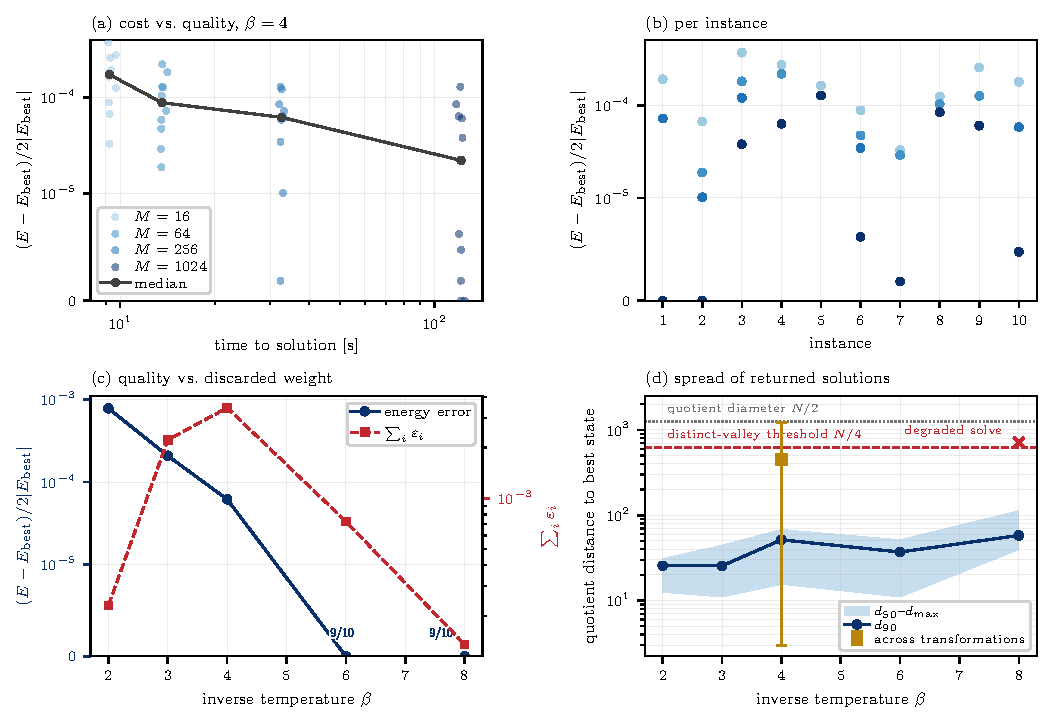
\includegraphics[width=\linewidth]{quality.pdf}
\caption{Ten 2500-spin ($50\times50$) square-lattice instances at bond dimension
8 on CPU. (a) Time to solution versus relative energy error as
$M=$~\texttt{max\_states} varies from 16 to 1024. Points show individual
instances. The line shows their median. (b) The same measurements indexed by
instance. (c) Median energy error and aggregate discarded weight
$\sum_i\varepsilon_i$ versus $\beta$. Labels count instances that reached the
best energy found. $E_{\mathrm{best}}$ is the lowest energy over all settings
shown, not a certified optimum. (d) Solution spread at $M=1024$, measured by
quotient distance $\min(d,N-d)$ to identify exact global spin-flip pairs. The
band and line show medians over ten instances of the 50th, 90th and 100th
percentiles of distance from each returned state to the best state. Squares
summarize pairwise minimum, median and maximum distances among eight
transformation results at $\beta=4$ over five instances. Supplementary
Section~\ref{sec:supp-diversity} provides definitions, per-instance data and
analysis of the $\beta=8$ outlier.}
\label{fig:evr}
\end{figure}
\FloatBarrier

\subsection{Transformation sweeps and hardware performance}

The standard protocol applies each lattice transformation once per instance.
Previously, users implemented this loop. \texttt{sweep\_transformations} now
seeds each transformation deterministically because \texttt{Zipper} draws a
random sketch and task scheduling can otherwise affect results. It also isolates
failures and reports the diagnostics described above. Available device memory
limits concurrency. A calibration solve measures peak memory, and admission is
controlled by a byte budget. Each admitted solve receives a task-local
reservation used to size its kernel batches. Concurrent solves therefore cannot
each size batches against the full shared memory pool.

Concurrent execution reduced sweep time on both CPU and GPU
(Table~\ref{tab:sweep}). CPU speed-up increased monotonically to $3.1\times$ and
$1.6\times$ at $c=8$ for the two cases. GPU speed-up reached $1.7\times$ at
$c=2$ and $1.4\times$ at $c=4$. At $c=1$, fixed sweep setup increased wall time
because no solves overlapped. Energies agreed for every configuration. All
ratios use the paired, interleaved protocol summarized in the table caption and
documented in Supplementary Section~\ref{sec:supp-timing}.

\begin{table}[!htbp]
\small
\centering
\caption{Speed-up of the concurrent sweep over the serial eight-transformation loop.
Each entry is the median of per-round paired ratios, measured with interleaved arms
and a full reclaim before every timed section. Intel Xeon Platinum 8462Y+ (CPU, 5
rounds) and one NVIDIA H100 (GPU, 7 rounds). n.m. indicates not measured.}
\label{tab:sweep}
\begin{tabular}{@{}llcccc@{}}
\toprule
Case & Device & $c{=}1$ & $c{=}2$ & $c{=}4$ & $c{=}8$ \\
\midrule
Chimera $3\!\times\!4\!\times\!3$, $D{=}16$ & CPU & 0.88 & 1.41 & 2.14 & \textbf{3.09} \\
Chimera 128-spin, $D{=}32$, \texttt{Zipper} & CPU & 0.89 & 1.11 & 1.31 & \textbf{1.64} \\
Chimera $3\!\times\!4\!\times\!3$, $D{=}16$ & GPU & 0.91 & \textbf{1.69} & 1.44 & n.m. \\
Chimera 128-spin, $D{=}32$, \texttt{Zipper} & GPU & 0.83 & 1.22 & \textbf{1.43} & n.m. \\
\bottomrule
\end{tabular}
\end{table}

The original article recommends GPU execution for larger examples. On the tested
Xeon/H100 system, matched CPU and GPU configurations gave shorter GPU wall time
in only one measured cell (Figure~\ref{fig:cross}). CPU wall time was about
$45\times$ shorter at 36 spins.
At 2048 spins and $D=16$, it was about $1.6\times$ shorter for the dense instance
and $1.3\times$ shorter for the sparse instance. GPU wall time was about
$1.4\times$ shorter only for the 2048-spin sparse instance at $D=32$. For the
dense instance at that size, CPU wall time remained about 10\% shorter. Energies
agreed in every measured cell. Supplementary
Table~\ref{tab:supp-crossover} reports all ratios and protocol details.

\begin{figure}[!htbp]
\centering
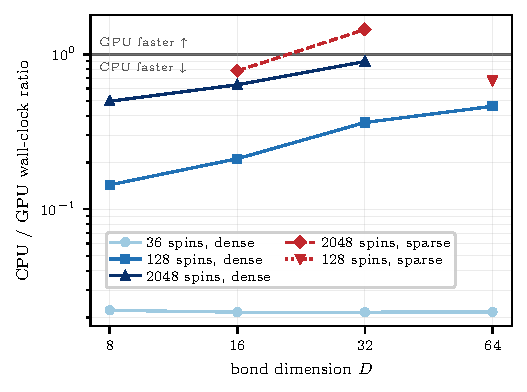
\includegraphics[width=0.62\linewidth]{crossover.pdf}
\caption{CPU/GPU wall-clock ratio on identical configurations. Ratios below one
indicate shorter CPU wall time. A ratio above one occurred only for the
2048-spin sparse instance at $D=32$. Measurements used \texttt{Zipper},
\texttt{SquareSingleNode}, $\beta=3$ and \texttt{max\_states}${=}128$ on an
Intel Xeon Platinum 8462Y+ and one NVIDIA H100. Supplementary
Table~\ref{tab:supp-crossover} reports the complete values.}
\label{fig:cross}
\end{figure}
\FloatBarrier

\subsection{Profiling and allocation}

On a profiled 128-spin solve, host-side CUDA API calls covered 27.0\% of the
profiled span and GPU activities covered 6.6\%. These intervals may overlap, so
at least 66.5\% of the span lay outside the two recorded categories. This large
host interval is consistent with the measured CPU/GPU crossover. Faster tensor
kernels do not reduce host-side bookkeeping.

Kernel-level batching could reduce device idle time. We did not implement it
because eliminating the entire measured CUDA API share gives an Amdahl-style
upper bound of about $1.4\times$ for this profile. Host allocation could be
reduced directly. In the published code, \texttt{branch\_states} accounted for
52.7\% of the bytes allocated by a 128-spin solve. This motivated two changes
(Figure~\ref{fig:alloc}). First, a single matrix now stores branched
configurations instead of tens of thousands of small vectors per call. Allocated
bytes fell by about 4\% in the large GPU run and 1\% in the corresponding CPU
run. The main effect is a lower live-object count. Second, multi-tensor
contraction temporaries moved from the collected heap to explicit allocation.
This reduced allocated bytes for a 2048-spin, bond-32 CPU solve by about two
thirds, from 90.9 to 32~GiB. Both changes were measured in a full solve. The
explicit allocator was not faster in isolation. Its benefit comes from removing
allocations from the collected heap.

\begin{figure}[H]
\centering
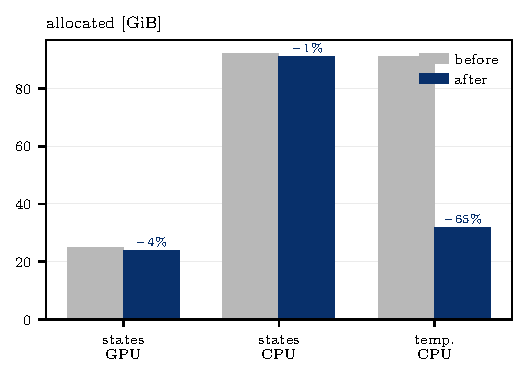
\includegraphics[width=\linewidth]{allocation.pdf}
\caption{Allocated memory before and after the two allocation changes, on a
2048-spin bond-32 solve, with percentages giving the reduction. ``states'' is
the matrix-backed branched configuration set and ``temp.'' the off-heap
contraction temporaries. Moving the temporaries reduced CPU heap allocation by
about two thirds. The states change has a small effect on allocated \emph{bytes}
because it primarily reduces the live-object count. The post-change totals were
32.3~GiB on CPU and 24.1~GiB on GPU on the H100 test system.}
\label{fig:alloc}
\end{figure}
\FloatBarrier

\subsection{Impact, limitations and outlook}

The new diagnostic exposes substantial truncation loss in cold contractions when
no exact answer is available, the regime the method targets. The consolidation
and the deprecation shims make the published interface reproducible, and
shipping the benchmark instances closes a gap in that reproducibility that
predates this update. Supplementary
Section~\ref{sec:supp-reproducibility} maps the additional results to their
drivers and committed records. The arXiv ancillary
\texttt{anc/benchmarks/} directory contains the raw per-run data, figure scripts
and runnable drivers for the crossover, concurrency, diversity,
energy-vs-runtime, contraction-error and $\beta$-ladder results. The allocation
figure's pre-change values are recorded measurements of the superseded code.

Warm starting currently covers only the bottom boundary MPS, so layouts that
build the top boundary do not benefit on those rows. $\sum\varepsilon$ did not
select $\beta$ in our tests. The package therefore documents it as a diagnostic
rather than a selection criterion.


%% Keep pending floats before the reference list without forcing a page break.
\FloatBarrier

\appendix
\setcounter{section}{0}
\setcounter{table}{0}
\setcounter{equation}{0}
\renewcommand{\thesection}{S\arabic{section}}
\renewcommand{\thesubsection}{\thesection.\arabic{subsection}}
\renewcommand{\thetable}{S\arabic{table}}
\renewcommand{\theequation}{S\arabic{equation}}
\renewcommand{\theHsection}{supp.\arabic{section}}
\renewcommand{\theHtable}{supp.\arabic{table}}
\renewcommand{\theHequation}{supp.\arabic{equation}}
\newcommand{\suppdatadir}{\path{anc/benchmarks/}}
\newcommand{\suppfile}[1]{\path{anc/benchmarks/#1}}
\section*{Supplementary material}
% This file is shared verbatim by the SoftwareX supplement and arXiv appendix.
% Numbering is configured by the including document.

\section{Matched CPU and GPU measurements}
\label{sec:supp-crossover}

Table~\ref{tab:supp-crossover} compares matched CPU and GPU wall times for
identical solver configurations. Ratios are CPU wall time divided by GPU wall
time. CPU and GPU measurements alternated, with each run executed in a separate
process on an Intel Xeon Platinum 8462Y+ and one NVIDIA H100. All measurements
used \texttt{Zipper}, \texttt{SquareSingleNode}, $\beta=3$, and
\texttt{max\_states}=128. Search breadth was fixed to isolate device-dependent
contraction work. The branch-and-bound search runs on the host in both arms. The
36- and 128-spin cases used seven repetitions per device. The 2048-spin cases
used two because of their higher computational cost. The summary uses the
minimum wall time for each arm.

\begin{table}[htbp]
\small
\centering
\caption{CPU/GPU wall-clock ratios for matched configurations. A value below
one indicates shorter CPU wall time. n.m. indicates not measured.}
\label{tab:supp-crossover}
\begin{tabular}{@{}lcccc@{}}
\toprule
Spins and structure & $D{=}8$ & $D{=}16$ & $D{=}32$ & $D{=}64$ \\
\midrule
36, dense     & 0.02 & 0.02 & 0.02 & 0.02 \\
128, dense    & 0.14 & 0.21 & 0.36 & 0.46 \\
128, sparse   & n.m. & n.m. & n.m. & 0.68 \\
2048, dense   & 0.50 & 0.64 & 0.90 & n.m. \\
2048, sparse  & n.m. & 0.78 & \textbf{1.45} & n.m. \\
\bottomrule
\end{tabular}
\end{table}

GPU wall time was shorter only for the 2048-spin sparse instance at $D=32$.
Energies agreed in every measured cell. Raw per-run measurements are stored in
\suppfile{crossover_raw.csv}. The summarized CPU and GPU times and their ratios
are stored in \suppfile{crossover.csv}.
\FloatBarrier

\section{Solution-diversity analysis}
\label{sec:supp-diversity}

The diversity experiments used 2500-spin square-lattice instances without local
fields, so every state $\sigma$ and its global spin flip $-\sigma$ have exactly
the same energy. To avoid counting this symmetry-related pair as two valleys,
distances are reported as
\[
    d_{\mathbb{Z}_2}(\sigma,\tau)
    = \min\!\left(d_H(\sigma,\tau),N-d_H(\sigma,\tau)\right),
\]
where $d_H$ is Hamming distance and $N=2500$. The largest possible quotient
distance is $N/2=1250$. The diversity criterion used in the original article is
$N/4=625$.

Of the 50 instance-temperature runs tested at \texttt{max\_states}=1024, 49
remained within one valley. Across those runs, the largest quotient distance
between any returned state and the best returned state was 399. The sole
exception was instance 1 at $\beta=8$. Its best returned energy was 8.12 above
the lowest energy among the five fixed-order $\beta$ runs for that instance. No
returned state was the global spin flip of the best returned state. We interpret
this result as a degraded contraction rather than evidence of an additional
low-energy valley.

Varying the contraction order broadened the solution set. At $\beta=4$,
selecting one state from each of the eight lattice transformations yielded two
or three distinct valleys on four of five instances. Pairwise quotient distances
reached 1249, compared with the maximum possible value of 1250. Across the same
transformations, the relative energy spread ranged from $2.21\times10^{-4}$ to
$5.74\times10^{-4}$.

The per-run distance quantiles are stored in \suppfile{div3.csv} and
\suppfile{div3_extra.csv}. The per-instance cross-transformation measurements
are in \suppfile{xtransform.csv}. Panel (d) of Figure~1 in the main article
reports medians over ten instances of the 50th, 90th, and 100th within-run
distance percentiles. At $\beta=4$, the square marks the median across five
transformation-sweep instances of the pairwise median distance. Its error bars
extend to the corresponding medians of the pairwise minimum and maximum.

\begin{table}[htbp]
\scriptsize
\centering
\caption{Per-run quotient-distance summaries. Each entry gives
$d_{50}/d_{90}/d_{\max}$ for the 1024 states returned in one fixed-order run.}
\label{tab:supp-diversity-runs}
\begin{tabular}{@{}crrrrr@{}}
\toprule
Instance & $\beta=2$ & $\beta=3$ & $\beta=4$ & $\beta=6$ & $\beta=8$ \\
\midrule
1  & 24/27/31 & 11/15/17 & 7/89/105 & 18/143/145 & 684/702/711 \\
2  & 15/24/31 & 9/143/154 & 20/144/156 & 138/153/164 & 129/152/166 \\
3  & 6/13/29 & 11/19/24 & 10/165/180 & 12/41/66 & 12/40/66 \\
4  & 50/78/94 & 257/293/308 & 8/37/44 & 7/12/52 & 8/13/51 \\
5  & 17/48/63 & 46/60/191 & 42/51/189 & 12/51/190 & 8/45/152 \\
6  & 4/10/13 & 7/13/399 & 10/14/17 & 4/8/11 & 67/71/74 \\
7  & 8/13/19 & 8/12/19 & 32/37/42 & 6/10/13 & 323/329/333 \\
8  & 17/39/45 & 14/27/35 & 28/52/65 & 22/33/40 & 12/19/24 \\
9  & 10/27/32 & 9/24/52 & 15/41/48 & 6/46/51 & 349/352/371 \\
10 & 9/16/26 & 18/28/37 & 16/64/71 & 10/17/23 & 10/17/23 \\
\bottomrule
\end{tabular}
\end{table}

\begin{table}[htbp]
\small
\centering
\caption{Per-instance results across eight lattice transformations at
$\beta=4$. The energy spread is the maximum minus minimum returned energy.
Distances are pairwise quotient distances.}
\label{tab:supp-transform-diversity}
\begin{tabular}{@{}crrrrrrr@{}}
\toprule
Instance & Consensus & $\Delta E$ &
$10^4\Delta E/|E_{\mathrm{best}}|$ &
$d_{\min}$ & $d_{\mathrm{med}}$ & $d_{\max}$ & Valleys \\
\midrule
1 & 1/8 & 0.7815 & 4.02 & 19 & 820 & 1214 & 3 \\
2 & 1/8 & 1.1294 & 5.74 & 21 & 450 & 1249 & 2 \\
3 & 2/8 & 0.4531 & 2.30 & 0  & 971 & 1226 & 2 \\
4 & 1/8 & 0.4309 & 2.21 & 3  & 86  & 686  & 2 \\
5 & 1/8 & 0.4998 & 2.56 & 0  & 212 & 355  & 1 \\
\bottomrule
\end{tabular}
\end{table}
\FloatBarrier

\section{Timing protocol and CUDA memory-pool artifact}
\label{sec:supp-timing}

\subsection{Paired measurements}

The concurrent-sweep and inverse-temperature-ladder comparisons use paired
measurements. The two arms are interleaved within each round. The concurrency
driver performs a full \texttt{GC.gc(true)} before each timed section, followed
by \texttt{CUDA.reclaim()} for device measurements. The ladder driver performs
the same host reclamation before each complete cold or warm arm. Reported
speed-ups are medians of the per-round paired ratios.

The ladder benchmark used the 2048-spin sparse instance at $D=16$ with five
rounds and seeds 2 through 6. Each round ran one cold and one warm ladder on
fresh contractors. Their order alternated across rounds. Rung 1 was cold in
both arms. Rungs 2 and 3 reused a retained boundary MPS only in the warm arm.
Table~\ref{tab:supp-ladder} reports the paired timing ratios. Median discarded
weights for the cold arm were $3.203543\times10^{-3}$,
$1.686507\times10^{-4}$, and $1.856007\times10^{-5}$ over the three rungs. The
warm arm matched the first value and recorded zero for rungs 2 and 3 because a
warm start does not perform a truncating factorization. The returned rung
energies were $-3334.080055$, $-3336.773383$, and $-3336.773383$.

\begin{table}[htbp]
\footnotesize
\centering
\caption{Five-round inverse-temperature-ladder benchmark. Ratios are cold-arm
wall time divided by warm-arm wall time. The interval gives the minimum and
maximum paired ratios. Reduction is $1-1/r$, where $r$ is the median ratio.}
\label{tab:supp-ladder}
\begin{tabular}{@{}cclccc@{}}
\toprule
Rung & $\beta$ & Initialization &
Median ratio & Ratio interval & Reduction \\
\midrule
1 & 1.50 & cold in both arms & 1.008 & [0.916, 1.091] & 0.8\% \\
2 & 2.25 & retained boundary MPS & 1.323 & [1.240, 1.440] & 24.4\% \\
3 & 3.00 & retained boundary MPS & 1.341 & [1.273, 1.730] & 25.4\% \\
\midrule
\multicolumn{3}{l}{Complete ladder} &
1.188 & [1.115, 1.349] & 15.8\% \\
\bottomrule
\end{tabular}
\end{table}

\subsection{Timing contamination checks}

A misleading result from a sequential protocol motivated the paired design. We
retained its summary values, but not the raw development log. A concurrent
warm-up left the CUDA memory pool in a different state when the serial arm was
timed.
For identical work, the serial baseline rose from 14.3~s to 38.8~s, a factor of
approximately 2.7. The contaminated baseline implied a speed-up of
$1.68\times$, whereas the corrected paired protocol gave $0.92\times$. All
reported sweep and ladder ratios use the interleaved protocol and reclamation
steps above.

The crossover experiment uses alternating separate processes. Each process
receives an uncontended device, and the summary uses the minimum of its repeated
wall-time measurements. Timing runs were performed on an otherwise idle
machine.

An exploratory benchmark run coincided with the full package test suite and
returned a different energy at one of 30 benchmark points. We excluded that run
because the machine was not idle. The cause of the difference remains unresolved.
\FloatBarrier

\section{Reproducibility inventory}
\label{sec:supp-reproducibility}

The drivers use the \texttt{SpinGlassPEPS.jl} v2.0.1 API. The launcher runs the
local checkout selected by \texttt{PKG}. To reproduce the article values, check
out the v2.0.1 tag before launching the complete suite from the supplementary
\suppdatadir{} directory with

\begin{verbatim}
PKG=../../SpinGlassPEPS.jl GPU=0 SEED=1 ./run_all.sh
\end{verbatim}

The energy/runtime and fixed-order diversity drivers use
\texttt{SEED + instance}, reset the random stream before each solve, and record
the derived seed in every CSV row. Matching parameter settings use the same
random stream independently of loop order.

The launcher instantiates the package environment, runs the measurement drivers,
writes raw and summarized CSV files, and regenerates the figures.
Table~\ref{tab:supp-inventory} maps the reported results to their drivers and
committed records.

\begin{table}[htbp]
\footnotesize
\centering
\caption{Inventory of supplementary drivers and committed result files.}
\label{tab:supp-inventory}
\begin{tabular}{@{}p{0.24\linewidth}p{0.30\linewidth}p{0.38\linewidth}@{}}
\toprule
Result & Driver or processor & Committed records \\
\midrule
Energy, runtime, and diversity
  & \path{sweep50.jl}, \path{spread.jl}, \path{xtransform.jl}
  & \path{sweep50_cpu.csv}, \path{div3.csv},
    \path{div3_extra.csv}, \path{xtransform.csv} \\
CPU/GPU crossover
  & \path{crossover.jl}, \path{summarize_crossover.py}
  & \path{crossover_raw.csv}, \path{crossover.csv} \\
Concurrent transformation sweep
  & \path{concurrency.jl}, \path{summarize_concurrency.py}
  & \path{concurrency_raw.csv}, \path{concurrency.csv} \\
Allocation and profiling
  & \path{alloc.jl}, \path{profile.jl}
  & \path{alloc_raw.csv}, \path{alloc.csv}, \path{profile.csv} \\
Discarded-weight diagnostics
  & \path{eps_stats.jl}
  & \path{eps_stats.csv} \\
Inverse-temperature ladder
  & \path{ladder.jl}
  & \path{ladder_raw.csv} \\
Figure generation
  & \path{makefigs.py}
  & \path{figures/quality.pdf}, \path{figures/crossover.pdf},
    \path{figures/allocation.pdf} \\
\bottomrule
\end{tabular}
\end{table}

The 36-spin, 128-spin, and 2048-spin instances are distributed in
\path{test/engine/instances/} of the package. The recovered 2500-spin instances
are in \path{benchmark/instances/square_50x50/}. Crossover, concurrency,
post-change allocation, profiling, and ladder measurements used an Intel Xeon
Platinum 8462Y+ system. GPU measurements used one NVIDIA H100.
A multithreaded run reproduced \path{xtransform.csv} byte for byte. Its output
is stored as \path{xtransform_multithread.csv}. The discarded-weight calculation
recorded in \path{eps_stats.csv} ran on the CPU.

\subsection{Discarded-weight record}

Table~\ref{tab:supp-eps} gives the complete diagnostic record used for the
128-spin example in the main article. A truncation is counted as bond-limited
only when the bond cap discards relative weight above $10^{-12}$.

\begin{table}[htbp]
\scriptsize
\centering
\caption{Discarded-weight diagnostics for the 128-spin test instance.}
\label{tab:supp-eps}
\begin{tabular}{@{}crrrrr@{}}
\toprule
$D$ & $\sum_i\varepsilon_i$ & $\max_i\varepsilon_i$ &
Bond-limited & Retained/offered & Energy \\
\midrule
4  & $3.148221\times10^{-4}$ & $2.425283\times10^{-4}$ &
18/18 & 108/307 & $-210.933334$ \\
32 & $5.564114\times10^{-14}$ & $5.511773\times10^{-14}$ &
0/4 & 192/592 & $-210.933334$ \\
\bottomrule
\end{tabular}
\end{table}

\subsection{Allocation provenance}

The pre-change allocation values in Figure~3 of the main article measure
superseded code and cannot be regenerated from v2.0.0. They are retained in
\suppfile{alloc.csv}. Their development code state and protocol are documented
in \suppfile{README.md}. The supplied driver regenerates the final combined
v2.0.0 totals in \suppfile{alloc_raw.csv}.
Table~\ref{tab:supp-allocation} reports the committed isolated-change records in
\suppfile{alloc.csv}. \suppfile{run_all.sh} does not regenerate every
post-change arm in that file.

\begin{table}[htbp]
\small
\centering
\caption{Allocated-memory measurements used in Figure~3 of the main article.}
\label{tab:supp-allocation}
\begin{tabular}{@{}lrrrr@{}}
\toprule
Change & Device & Before [GiB] & After [GiB] & Reduction \\
\midrule
Matrix-backed branched states & GPU & 25.05 & 23.96 & 4.35\% \\
Matrix-backed branched states & CPU & 92.06 & 91.05 & 1.10\% \\
Off-heap temporaries & CPU & 90.9 & 32.0 & 64.80\% \\
\bottomrule
\end{tabular}
\end{table}
\FloatBarrier

\section{Correctness regression coverage}
\label{sec:supp-correctness}

The two result-affecting defects described in the article are covered by
dedicated regression tests. Tests in
\path{test/tensors/contractions_site.jl} and
\path{test/tensors/contractions_virtual.jl} compare
\texttt{corner\_matrix} outputs with independently constructed dense references.
They verify output dimensions and numerical values on CPU and GPU.

The exhaustive-search regression in \path{test/exhaustive/ising.jl} uses a
deterministic ten-spin instance. It compares all 1024 GPU state codes and their
energies with complete CPU enumeration. The GPU launch uses 512 threads per
block, so this test exercises two blocks and crosses the boundary that exposed
the former incomplete-spectrum defect. GPU regression tests run when CUDA is
functional. CPU test groups remain available on systems without a CUDA-capable
device.

\FloatBarrier

\section*{CRediT authorship contribution statement}

\noindent\textbf{{\L}ukasz Pawela:} Conceptualization, Formal analysis, Funding
acquisition, Investigation, Methodology, Project administration, Resources,
Software, Supervision, Validation, Writing -- original draft, Writing -- review
\& editing.

\noindent\textbf{Bart\l{}omiej Gardas:} Conceptualization, Formal analysis,
Funding acquisition, Investigation, Methodology, Project administration,
Resources, Software, Supervision, Writing -- original draft, Writing -- review
\& editing.

\section*{Declaration of competing interest}

The authors report financial support from the National Science Centre, Poland,
as stated in the Acknowledgements. They declare no other known competing
financial interests or personal relationships that could have appeared to
influence the work reported in this paper.

\section*{Data availability}

The version 2.0.0 source code and benchmark instances are archived on
Zenodo~\cite{spinglasspeps_zenodo}. The available benchmark records, drivers and
plotting scripts supporting the reported results are included in the arXiv
ancillary files under \path{anc/benchmarks/}. Raw logs for the historical
pre-change allocation measurements were not retained. The corresponding summary
values and protocol context are included.

\section*{Acknowledgements}
\label{acknowledgements}

This work was supported by the National Science Centre (NCN), Poland, through
SONATA BIS 10, grant no.~2020/38/E/ST3/00269 (B.G.), and SONATA BIS 15, grant
no.~2025/58/E/ST6/00422 ({\L}.P.).

\bibliographystyle{elsarticle-num}
\bibliography{refs}

\end{document}
